%
% Copyright (c) 2011-2013, fortiss GmbH.
% Licensed under the Apache License, Version 2.0.
% 
% Use, modification and distribution are subject to the terms specified
% in the accompanying license file LICENSE.txt located at the root directory
% of this software distribution. A copy is available at
% http://chromosome.fortiss.org/.
%
% This file is part of CHROMOSOME.
%
% $Id$
%

% =================================================================
\section{Example 6: Consumer with Queue (10 minutes)}
\label{sec:example_queues}
% =================================================================

This is a simple example of queues used in a subscription.
To look at it, import the \textit{queues} example into XMT,
as you have previously done it with the \emph{sensorMonitor} example (see Section~\ref{sec:example_xmt}).

Queues on a subscription become necessary when multiple data items are sent to it,
before its function(s) can process the previous data item.
In this example there are two sender components and one receiver component on the same node.
Each sender component has a single publication, and each receiver has a subscription.
Therefore two local routes will be constructed that are connected to the subscription.
Each sender is executed at a frequency of 1.5~Hz, whereas the receiver is executed twice as often at a frequency of 3.0~Hz.
Therefore the receiver will in principle be executed often enough to consume all data items.
But it might happen that multiple data items arrive in the same cycle.
In this example the senders will each be executed in every other cycle,
so that two data items arrive at the receiver in that cycle.
The problem is that in a single cycle the receiver will only process a single data item.
To resolve this, the subscription of the receiver has its queue size set to \textit{2}, see screenshot~\ref{fig:example_queues_manifest}.
So in the subsequent cycle, the receiver will process the second data item (no new data items arrive),
which has been buffered in the queue.

\begin{figure}[htpb]
	\centering
	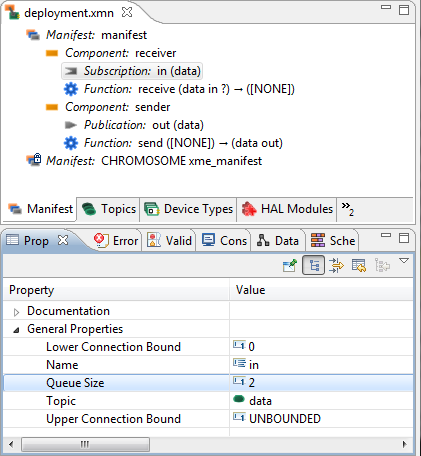
\includegraphics[scale=0.75]{figures/example_queues_manifest.png}
	\caption{Manifest of queues example, highlighting the queue size.}
	\label{fig:example_queues_manifest}
\end{figure}

Screenshot~\ref{fig:example_queues} shows the console output from the example.
On execution you will notice a 3 second delay between each receiver execution.
Despite two data items arriving at once it will be able to process both items.
Without a queue the second data item would have overwritten the first.

\begin{figure}[htpb]
	\centering
	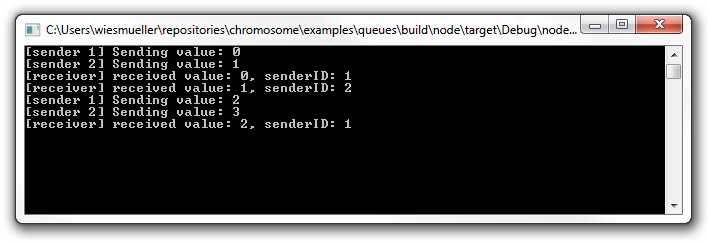
\includegraphics[scale=0.5]{figures/example_queues.png}
	\caption{Execution of queues example.}
	\label{fig:example_queues}
\end{figure}
